\documentclass[12pt]{article}

\newif\ifpdf
\ifx\pdfoutput\undefined
\pdffalse % not running PDFLaTeX
\else
\pdfoutput=1 % running PDFLaTeX
\pdftrue
\fi

\ifpdf
\usepackage[pdftex]{graphicx}
\else
\usepackage{graphicx}
\fi

%\usepackage[osf]{gtamachoefler}

% Added by bcarey
% Bibliography support
\usepackage{lscape}
\usepackage[super,comma,sort]{natbib}
%\usepackage[linux]{vpe}
%\vpesetup{noref}
%define citation punctuation style
\bibpunct[, ]{(}{)}{;}{a}{,}{,}

% Allow less text and more figure on page
\renewcommand{\topfraction}{0.90}
\renewcommand{\bottomfraction}{0.90}
\renewcommand{\textfraction}{0.1}
\renewcommand{\floatpagefraction}{0.90}

% end additions by bcarey


%\usepackage{times}
\usepackage{fourier}
\usepackage{sectsty,hangcaption}
\usepackage{amsmath,amsbsy,amssymb}
%\usepackage{deflist}
\usepackage{fancyhdr}
\usepackage{tabularx}
\usepackage{verbatim}
\usepackage{moreverb}
\usepackage{float}
\usepackage{fancybox}
\usepackage{graphicx}
\usepackage{longtable}
\usepackage{wrapfig}
\usepackage{booktabs}
\usepackage{comment}
%\usepackage{subfigure}

%must be last package
%\usepackage{hyperref}
\usepackage[debug=false, colorlinks=true, pdfstartview=FitV, linkcolor=blue, citecolor=blue, urlcolor=blue]{hyperref}

%\usepackage{toc_entr}
\textwidth 6.5in
\textheight 9.in
%\topmargin -0.75in
\topmargin -0.25in
%\topmargin -3.280cm
\newlength{\boxwidth}
\setlength{\boxwidth}{5.8in}
\oddsidemargin 0in
\evensidemargin 0in
\headheight 0.25in
\renewcommand{\thepage}{\arabic{section}--\arabic{page}}
%\lhead{ }
\lhead{}
\rhead{\today}
\chead{}
\cfoot{[\thepage]}
\lfoot{}
\rfoot{}
%\footrulewidth 0.4pt
\newcommand{\negsp}{\vspace{-4mm}}
\newcommand\secsp{\vspace{-3 mm}}
\newcommand\secspb{\vspace{-2 mm}}
\newcommand\subsecsp{\vspace{-0.0 mm}}
\renewcommand{\baselinestretch}{.9}
%\setlength{\baselineskip}{13pt}
\def\EQ#1\EN{\begin{equation}#1\end{equation}}
\def\BA#1\EA{\begin{align}#1\end{align}}
\def\BS#1\ES{\begin{split}#1\end{split}}
%\newcommand{\EQ}{\begin{equation}}
%\newcommand{\EN}{\end{equation}}
\newcommand{\longline}{\noindent\rule[-0.1in]{\textwidth}{0.01in}}
\newcommand{\bc}{\begin{center}}
\newcommand{\ec}{\end{center}}
\newcommand{\degc}{$^\circ$C}
\newcommand{\eq}{\ =\ }
\newcommand{\eff}{{\rm eff}}
\newcommand{\eqr}{{\rm le}}
\newcommand{\equ}{{\rm eq}}
\newcommand{\kin}{{\rm kin}}
\newcommand{\rdx}{{\rm rdx}}
\newcommand{\ind}{{\rm id}}
\newcommand{\dep}{{\rm dp}}
\newcommand{\e}{{\rm{e}}}
\newcommand{\erf}{{\rm{erf}}}
\newcommand{\erfc}{{\rm{erfc}}}
\newcommand{\sign}{{\rm{sign}}}
\newcommand{\p}{{\partial}}
\newcommand{\A}{{\mathcal A}}
\newcommand{\B}{{\mathcal B}}
\newcommand{\C}{{\mathcal C}}
\newcommand{\D}{{\mathcal D}}
\newcommand{\E}{{\mathcal E}}
\newcommand{\F}{{\mathcal F}}
\newcommand{\G}{{\mathcal G}}
\renewcommand{\H}{{\mathcal H}}
\newcommand{\I}{{\mathcal I}}
\newcommand{\J}{{\mathcal J}}
\newcommand{\jo}{{j_o}}
\newcommand{\M}{{\mathcal M}}
\newcommand{\cO}{{\mathcal O}}
\renewcommand{\P}{{{\mathcal P}}}
\newcommand{\Q}{{\mathcal Q}}
\newcommand{\R}{{{\mathcal R}}}
\renewcommand{\S}{{\mathcal S}}
\newcommand{\T}{{\mathcal T}}
\newcommand{\W}{{\mathcal W}}
\newcommand{\X}{{\mathcal X}}
\newcommand{\Y}{{\mathcal Y}}
\newcommand{\Z}{{\mathcal Z}}
\newcommand{\rev}{{\rm rev}}
\newcommand{\irr}{{\rm irr}}
\renewcommand{\a}{{\alpha}}
\newcommand{\abar}{{\bar \alpha}}
\renewcommand{\b}{{\beta}}
\newcommand{\w}{{\rm H_2O}}
\newcommand{\air}{{\rm N_2}}
\newcommand{\pe}{{\rm Pe}}
\newcommand{\da}{{\rm Da}}
\renewcommand{\k}{{\dot R}^0}
\renewcommand{\L}{\widehat{\mathcal L}}
\renewcommand{\bar}{\overline}
\newcommand{\dsty}{{\displaystyle}}
\newcommand{\diff}{{\mathcal D}}
\newcommand{\surf}{\equiv \!\!\!}
\newcommand{\bnabla}{\boldsymbol{\nabla}}
\newcommand{\bA}{\boldsymbol{A}}
\newcommand{\ba}{\boldsymbol{a}}
\newcommand{\bB}{\boldsymbol{B}}
\newcommand{\bC}{\boldsymbol{C}}
\newcommand{\bD}{\boldsymbol{D}}
\newcommand{\bE}{\boldsymbol{E}}
\newcommand{\bF}{\boldsymbol{F}}
\newcommand{\bi}{\boldsymbol{i}}
\newcommand{\bI}{\boldsymbol{I}}
\newcommand{\bJ}{\boldsymbol{J}}
\newcommand{\bK}{\boldsymbol{K}}
\newcommand{\blambda}{\boldsymbol{\lambda}}
\newcommand{\bM}{\boldsymbol{M}}
\newcommand{\bg}{\boldsymbol{g}}
\newcommand{\bGamma}{\boldsymbol{\Gamma}}
\newcommand{\bOmega}{\boldsymbol{\Omega}}
\newcommand{\bPsi}{\boldsymbol{\Psi}}
\newcommand{\bO}{\boldsymbol{O}}
\newcommand{\bnu}{\boldsymbol{\nu}}
\newcommand{\bn}{\boldsymbol{n}}
\newcommand{\bdS}{\boldsymbol{dS}}
\newcommand{\bq}{\boldsymbol{q}}
\newcommand{\br}{\boldsymbol{r}}
\newcommand{\bR}{\boldsymbol{R}}
\newcommand{\bS}{\boldsymbol{S}}
\newcommand{\bu}{\boldsymbol{u}}
\newcommand{\bv}{\boldsymbol{v}}
\newcommand{\bz}{\boldsymbol{z}}
\newcommand{\arrows}{~\rightleftharpoons~}
\newcommand{\arrowstab}{\!\!\!\rightleftharpoons\!\!\!}
\newcommand{\CA}{C_{\rm A}}
\newcommand{\CB}{C_{\rm B}}
\newcommand{\CC}{C_{\rm C}}
\newcommand{\CAB}{C_{\rm AB}}
\newcommand{\CBC}{C_{\rm BC}}
\newcommand{\RA}{\R_{\rm A}}
\newcommand{\RB}{\R_{\rm B}}
\newcommand{\RC}{\R_{\rm C}}
\newcommand{\RAB}{\R_{\rm AB}}
\newcommand{\RBC}{\R_{\rm BC}}
%\newcommand{\kdsc}{K^{DS}}
%\newcommand{\kdec}{K^{DE}}
%\newcommand{\kdsm}{\overline K^{DS}}
%\newcommand{\kdem}{\overline K^{DE}}
\newcommand{\kdsc}{K^{sc}}
\newcommand{\kdec}{K^{ec}}
\newcommand{\kdsm}{K^{sm}}
\newcommand{\kdem}{K^{em}}
\newcommand{\csm}{S}
\renewcommand{\csc}{S}
\newcommand{\cem}{\E}
\newcommand{\cec}{\E}
\renewcommand{\min}{{\rm min}}
\newcommand{\coll}{{\rm coll}}
\newcommand{\ex}{{\rm ex}}
\newcommand{\srf}{{\rm sc}}
\newcommand{\bGammah}{\hat{\bGamma}}
\newcommand{\Gammah}{\hat{\Gamma}}
\def\dbar{{\mkern2mu\mathchar'26\mkern-11mu\mathrm{d}}}

\newcounter{saveeqn}%
\newcommand{\alpheqn}{\setcounter{saveeqn}{\value{equation}}%
\stepcounter{saveeqn}\setcounter{equation}{0}%
\renewcommand{\theequation}
      {\mbox{\arabic{saveeqn}\alph{equation}}}}%
\newcommand{\reseteqn}{\setcounter{equation}{\value{saveeqn}}%
\renewcommand{\theequation}{\arabic{equation}}}%

\renewcommand{\contentsname}{Table of Contents}
\renewcommand{\listfigurename}{{List of Figures}}
\renewcommand{\listtablename}{{List of Tables}}

\renewcommand{\arraystretch}{1.3}

\setlength{\parindent}{0.3125in}
\setlength{\parskip}{2ex plus 0.2ex minus 0.2ex}

\setcounter{secnumdepth}{5}
\setcounter{tocdepth}{5}

\pagestyle{fancy}

\thispagestyle{empty}

%\renewcommand{\theequation}{\arabic{section}.\arabic{equation}}
%\renewcommand{\thetable}{{\arabic{section}.\arabic{table}}}
%\renewcommand{\thefigure}{{\arabic{section}.\arabic{figure}}}

\begin{document}


\subsection*{Conceptual Design of PETSc Time Stepper for Flow and Transport}
\addcontentsline{toc}{section}{Background}
\vspace{-16pt}
~
The generalized partial differential equation for groundwater flow is
\begin{equation}\label{flow}
\frac{\p}{\p t} \varphi\rho + \bnabla\cdot\rho\bu\eq \S,
\end{equation}
with $\bu$ given by Darcy's law
\begin{equation}\label{flux}
\bu\eq-\frac{\kappa}{\mu}\nabla\big(p-W\rho g z\big),
\end{equation}
with permeability $\kappa$, viscosity $\mu$, molar fluid density $\rho$, formula weight of water $W$, acceleration of gravity $g$, and source/sink term $\S$.  For full tensor permeability, permeability tensor $\kappa$ takes the form
\begin{equation}
\kappa \eq
\begin{bmatrix}
  k_{xx} & k_{xy} & k_{xz} \\
  k_{yx} & k_{yy} & k_{yz} \\
  k_{zx} & k_{zy} & k_{zz} \\
\end{bmatrix},
\end{equation}
and therefore, Equation \ref{flux} expands to
\begin{equation}
\bu \eq \dfrac{1}{\mu}
\begin{bmatrix}
  k_{xx} & k_{xy} & k_{xz} \\
  k_{yx} & k_{yy} & k_{yz} \\
  k_{zx} & k_{zy} & k_{zz} \\
\end{bmatrix}
\cdot
\renewcommand{\arraystretch}{2.5}
\begin{bmatrix}
  \dfrac{p}{\partial x} \\
  \dfrac{p}{\partial y} \\
  \dfrac{p-W\rho g z}{\partial z} \\
\end{bmatrix}.
\renewcommand{\arraystretch}{1}
\end{equation}
Since $\bu$ is the flux vector across the cells interface, $\bu$ could also be described as a scalar-vector product
\begin{equation}
\bu \eq
\begin{bmatrix}
  u_x \\
  u_y \\
  u_z \\
\end{bmatrix}
\eq u\cdot\bn \eq u\cdot
\begin{bmatrix}
  n_x \\
  n_y \\
  n_z \\
\end{bmatrix},
\end{equation}
where $\bn$ is a unit vector normal to the cell surface as shown in Figure \ref{schematic}.  Therefore,
\begin{equation}
u\cdot
\begin{bmatrix}
  n_x \\
  n_y \\
  n_z \\
\end{bmatrix}
\eq \dfrac{1}{\mu}
\begin{bmatrix}
  k_{xx} & k_{xy} & k_{xz} \\
  k_{yx} & k_{yy} & k_{yz} \\
  k_{zx} & k_{zy} & k_{zz} \\
\end{bmatrix}
\cdot
\renewcommand{\arraystretch}{2.5}
\begin{bmatrix}
  \dfrac{p}{\partial x} \\
  \dfrac{p}{\partial y} \\
  \dfrac{p-W\rho g z}{\partial z} \\
\end{bmatrix}.
\renewcommand{\arraystretch}{1}
\end{equation}



\begin{figure}[t]\centering
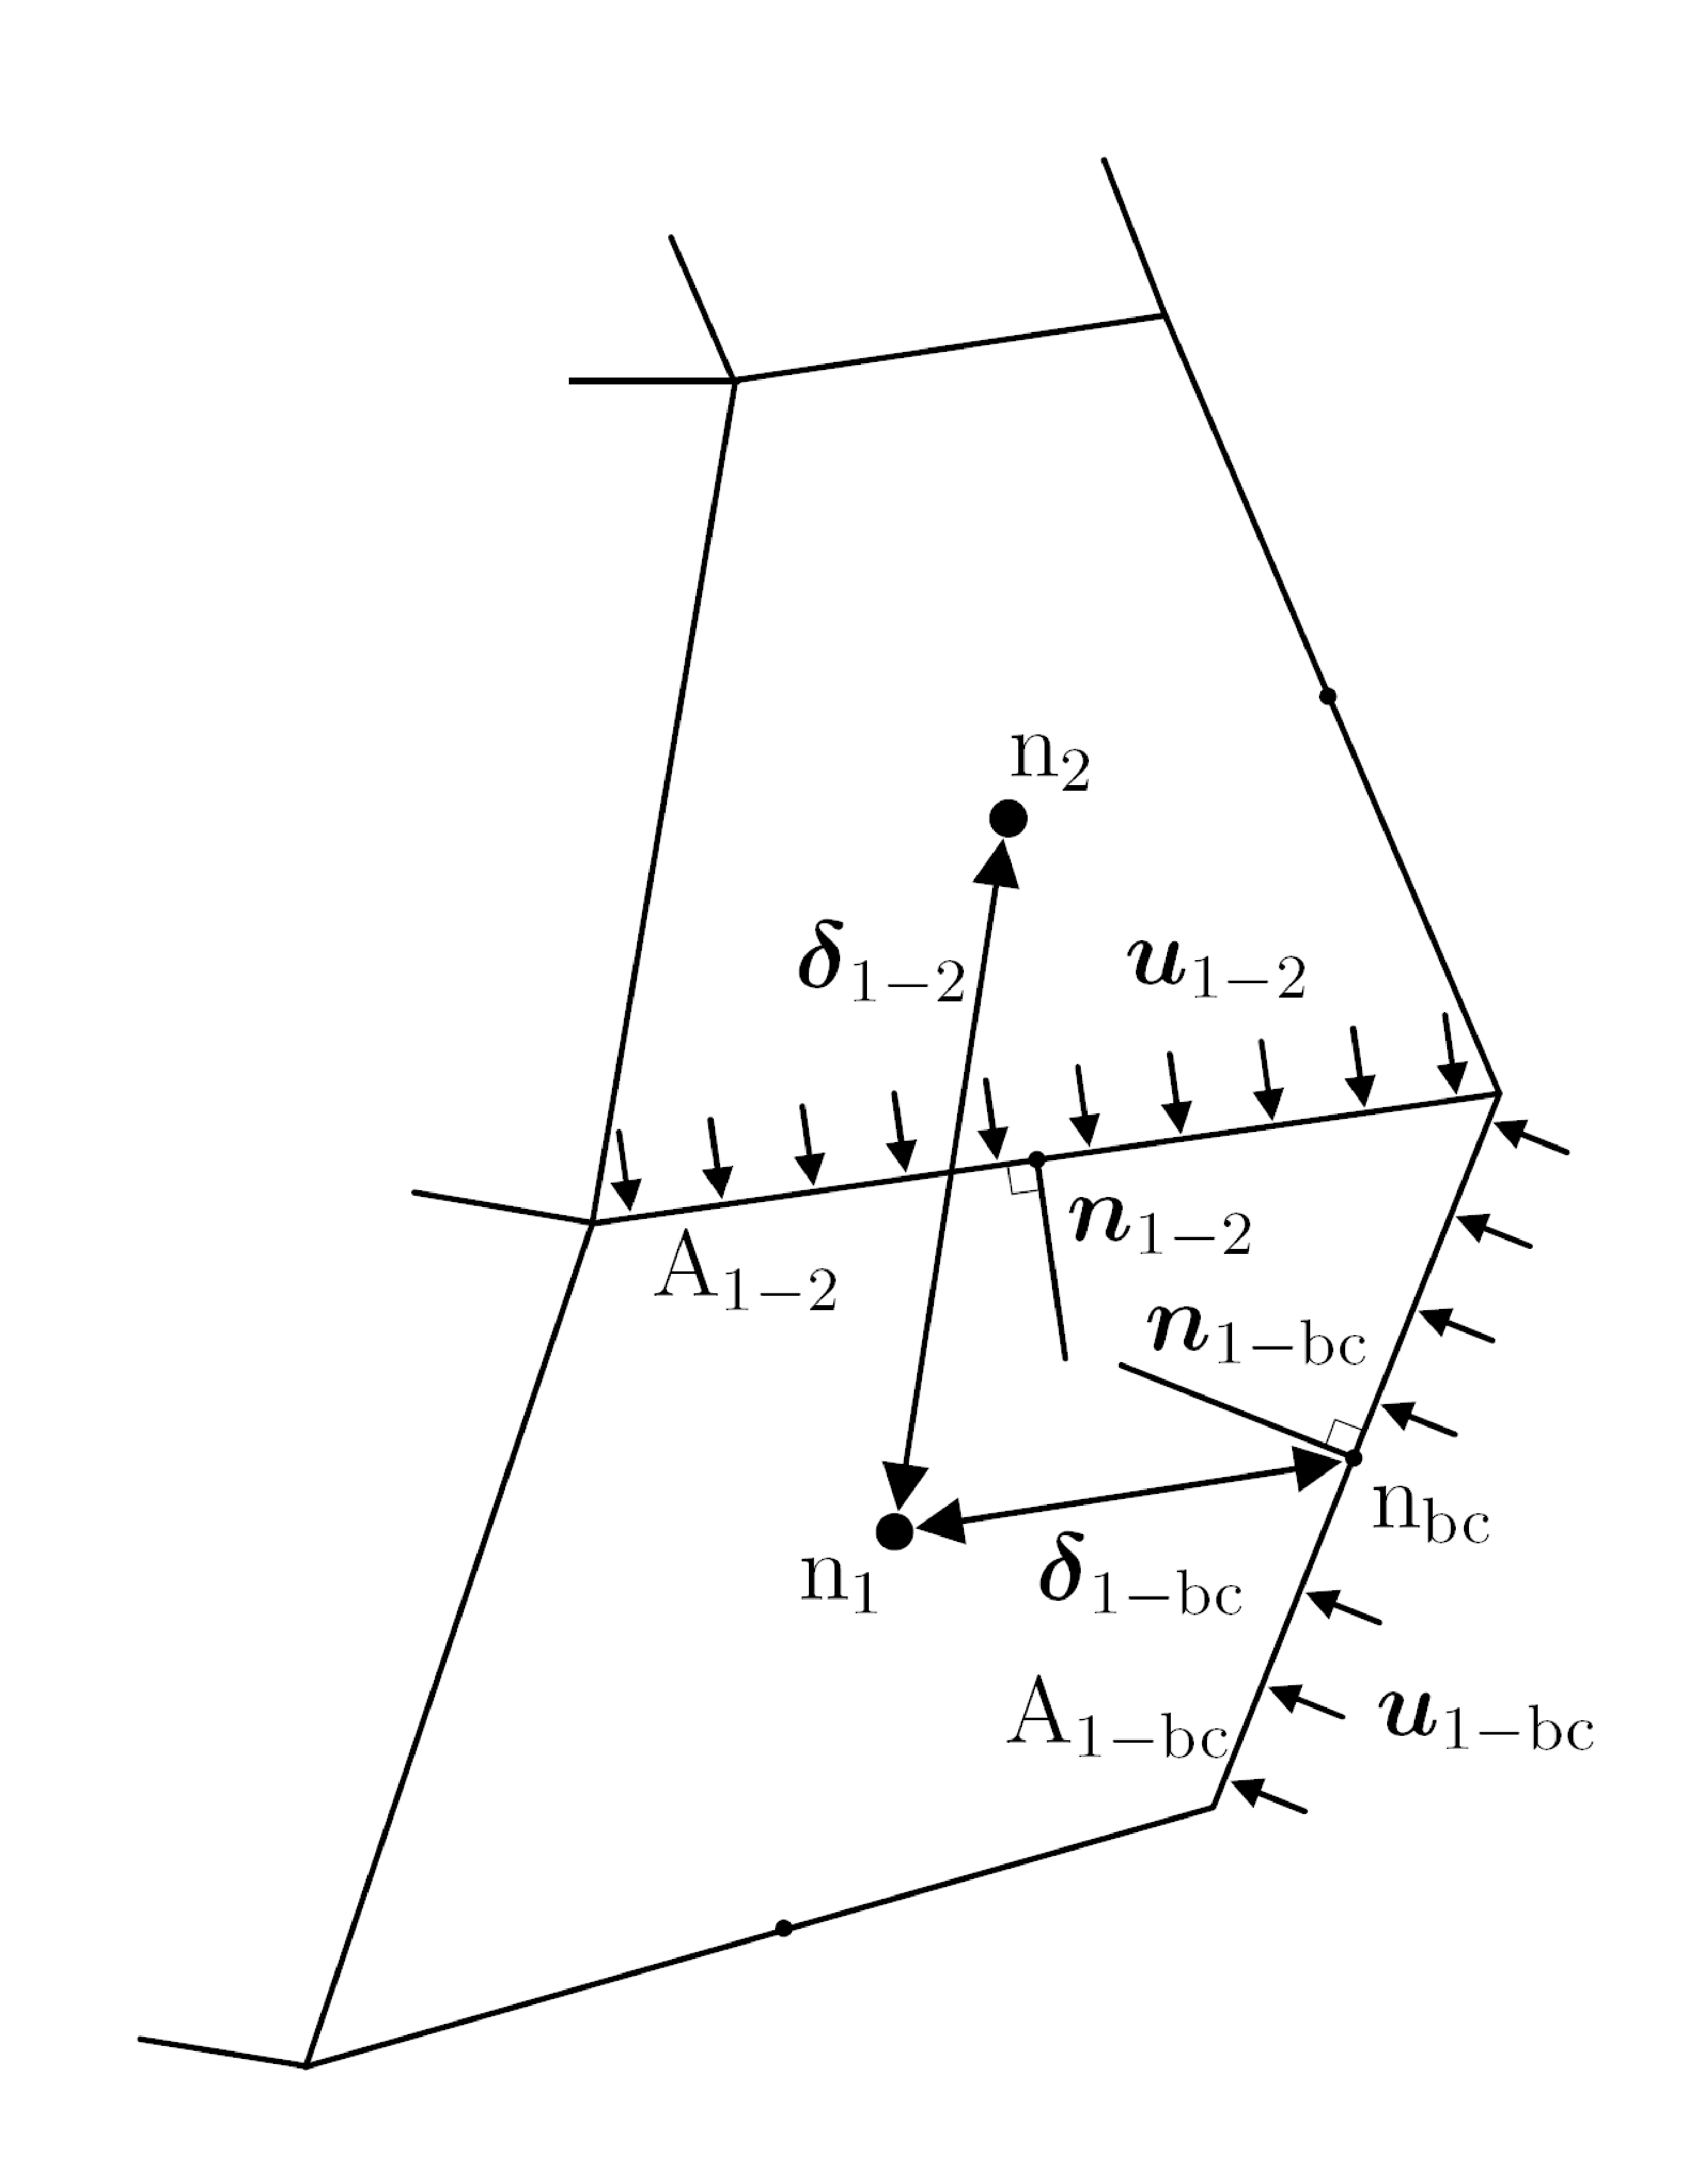
\includegraphics[width=3.0in]{./figs/Connection_Schematic2}
\caption{Schematic of unstructured grid.}
\label{schematic}
\end{figure}

The magnitude of the flux normal to the surface $(u)$ is obtained by multiplying through by $\bn^T$
\begin{equation}
u \eq \dfrac{1}{\mu}
\begin{bmatrix}
  n_x & n_y & n_z \\
\end{bmatrix}
\cdot
\begin{bmatrix}
  k_{xx} & k_{xy} & k_{xz} \\
  k_{yx} & k_{yy} & k_{yz} \\
  k_{zx} & k_{zy} & k_{zz} \\
\end{bmatrix}
\cdot
\renewcommand{\arraystretch}{2.5}
\begin{bmatrix}
  \dfrac{p}{\partial x} \\
  \dfrac{p}{\partial y} \\
  \dfrac{p-W\rho g z}{\partial z} \\
\end{bmatrix}.
\renewcommand{\arraystretch}{1}
\end{equation}
The scalar ''$u$'' is the flux applied across the boundary and intercellular fluxes in PFLOTRAN.
\end{document}
